\documentclass[12pt,a4paper]{article}

% Pacotes básicos
\usepackage[utf8]{inputenc}
\usepackage[T1]{fontenc}
\usepackage[brazil]{babel}
\usepackage{graphicx}
\usepackage{float}
\usepackage{amsmath, amssymb}
\usepackage{hyperref}
\usepackage{caption}
\usepackage{cite}

\graphicspath{{./}{../}{../../}{../../plots/}{../../plots/img/}}

\title{Relatório do Projeto de Grafos e Algoritmos de Busca}
\author{Grupo X \\ Disciplina Y \\ Universidade Z}
\date{\today}

\begin{document}

\maketitle
\tableofcontents
\newpage

\section{Introdução}
Nesta seção, deve ser apresentada uma visão geral do problema, os objetivos do relatório e uma breve descrição das tarefas realizadas. 
\cite{cormen}.

\section{Modelagem do Problema em Forma de Grafo}
O problema da \textit{Ponte e da Tocha} foi modelado como um problema de busca em espaço de estados e também como um CSP (\textit{Constraint Satisfaction Problem}). Essa abordagem permite tanto a análise formal do problema em termos de grafos, como também a aplicação de algoritmos de busca clássicos para encontrar soluções ótimas. 

A seguir, a modelagem será descrita em camadas: definição de estados, ações, função sucessora e custos.

\subsection*{Variáveis}

Para modelar o problema da ponte com $N$ pessoas como um COP, definimos um conjunto de variáveis de decisão. A variável principal é o tempo de travessia de cada pessoa, e as variáveis auxiliares nos ajudarão a definir a sequência de movimentos.

\begin{itemize}
    \item $t_i$: Variável que representa o tempo de travessia para a pessoa $i \in \{1, \dots, N\}$.
    \item $m_{i,j,k}$: Variável binária, onde $m_{i,j,k} = 1$ se as pessoas $i$ e $j$ atravessam a ponte juntas no passo $k$ (ida ou volta). Se apenas a pessoa $i$ atravessar, usamos $m_{i,0,k}$.
    \item $s_{i,k}$: Variável binária, onde $s_{i,k} = 1$ se a pessoa $i$ estiver no lado de partida (origem) após o passo $k$.
    \item $p_k$: Variável binária, onde $p_k=1$ se o passo $k$ é uma travessia de ida e $p_k=0$ se é uma travessia de volta.
\end{itemize}

\subsection*{Domínio das Variáveis}

\begin{itemize}
    \item $t_i \in \{T_1, T_2, \dots, T_N\}$, onde $T_i$ é o tempo individual da pessoa $i$.
    \item $m_{i,j,k} \in \{0, 1\}$.
    \item $s_{i,k} \in \{0, 1\}$.
    \item $p_k \in \{0, 1\}$.
\end{itemize}

\subsection*{Função Objetivo}
Nosso objetivo é minimizar o tempo total da travessia, que é a soma dos tempos de cada movimento.

$$
\min \sum_{k=1}^{K} \left( \sum_{i=1}^{N} \sum_{j=0}^{N} m_{i,j,k} \cdot \max(T_i, T_j) \right)
$$

Onde $T_0$ é o tempo de uma "pessoa imaginária" com tempo 0, para os casos de travessia única ($j=0$).
O número de passos $K$ pode ser estimado, mas não é fixo a priori.

\subsection*{Restrições}

\subsubsection*{Restrições de Movimento e Posição}
\begin{enumerate}
    \item \textbf{Apenas uma ação por passo:} Em cada passo $k$, apenas um movimento (conjunto de 1 ou 2 pessoas) é realizado.
    $$
    \sum_{i=1}^{N} \sum_{j=i}^{N} m_{i,j,k} + \sum_{i=1}^{N} m_{i,0,k} = 1 \quad \forall k
    $$
    \item \textbf{Consistência da Posição:} A posição de cada pessoa é atualizada a cada passo. Se a pessoa $i$ está no lado de partida ($s_{i,k-1}=1$) e se move para o lado de chegada ($m_{i,j,k}=1$), sua nova posição será de chegada ($s_{i,k}=0$).
    $$
    s_{i,k} = s_{i,k-1} + (p_k \cdot (\sum_{j=1}^{N} m_{i,j,k})) - ((1-p_k) \cdot (\sum_{j=1}^{N} m_{i,j,k})) \quad \forall i,k
    $$
    \item \textbf{Restrição da Tocha:} A direção da travessia deve se alternar. A tocha está sempre no lado oposto ao último movimento.
    $$
    p_k = 1 - p_{k-1} \quad \forall k > 1
    $$
\end{enumerate}

\subsubsection*{Restrições de Ação}
\begin{enumerate}
    \item \textbf{Posição da Tocha e Posição dos Atravessantes:} Apenas as pessoas no lado da tocha podem atravessar. Se o movimento é de ida ($p_k=1$), as pessoas devem estar no lado de partida ($s_{i,k-1}=1$). Se é de volta ($p_k=0$), elas devem estar no lado de chegada ($s_{i,k-1}=0$).
    $$
    m_{i,j,k} \cdot (1 - s_{i,k-1}) = 0 \quad \forall i, j, k \quad \text{(para travessia de ida)}
    $$
    $$
    m_{i,j,k} \cdot s_{i,k-1} = 0 \quad \forall i, j, k \quad \text{(para travessia de volta)}
    $$
    \item \textbf{Número de Pessoas por Travessia:} Apenas 1 ou 2 pessoas podem atravessar de cada vez.
    $$
    \sum_{i=1}^{N} \sum_{j=i}^{N} m_{i,j,k} + \sum_{i=1}^{N} m_{i,0,k} \in \{1, 2\} \quad \forall k
    $$
\end{enumerate}

\subsubsection*{Restrições de Conclusão}
\begin{enumerate}
    \item \textbf{Estado Inicial:} No início, todas as pessoas estão no lado de partida.
    $$
    s_{i,0} = 1 \quad \forall i \in \{1, \dots, N\}
    $$
    \item \textbf{Estado Final:} O problema é satisfeito quando, no passo final $K$, todas as pessoas estiverem no lado de chegada.
    $$
    s_{i,K} = 0 \quad \forall i \in \{1, \dots, N\}
    $$
\end{enumerate}

\subsection{Estados}
Seguindo a descrição do enunciado e visualizando a implementação em código, o estado do problema é representado por um array binário, que fornece uma representação compacta e eficiente.

\[
S = [p_1, p_2, p_3, p_4, t]
\]

Onde:
\begin{itemize}
    \item $p_i \in \{0, 1\}$ indica a posição da pessoa $i$ (A, B, C, D, respectivamente), onde $0$ representa o lado inicial (esquerdo) e $1$ representa o lado final (direito);
    \item $t \in \{0, 1\}$ indica a posição da tocha, onde $0$ representa o lado inicial e $1$ o lado final.
\end{itemize}

Assim, temos:
\begin{itemize}
    \item \textbf{Estado inicial}: $[0, 0, 0, 0, 0]$ (todas as pessoas e a tocha no lado inicial);
    \item \textbf{Estado objetivo}: $[1, 1, 1, 1, 1]$ (todas as pessoas e a tocha no lado final).
\end{itemize}

O lado final da ponte é implicitamente definido como o complemento do lado inicial.

\subsection{Ações e Função Sucessora}
Cada ação corresponde ao movimento de uma ou duas pessoas através da ponte, levando sempre a tocha consigo. A função sucessora gera todos os estados possíveis a partir de um estado atual, respeitando as regras do problema.

\begin{itemize}
    \item Se a tocha está no lado inicial ($t = 0$): escolher 1 ou 2 pessoas que estão no lado inicial ($p_i = 0$) para atravessar para o lado final;
    \item Se a tocha está no lado final ($t = 1$): escolher 1 ou 2 pessoas que estão no lado final ($p_i = 1$) para retornar ao lado inicial.
\end{itemize}

O custo de cada ação é definido como o tempo da travessia, que corresponde ao tempo da pessoa mais lenta entre as selecionadas.



\subsection{Exemplos Ilustrativos de Caminhos}
Para uma melhor clareza e visualização nos diagramas de grafo, os estados são representados utilizando a notação textual original, com o conjunto de pessoas no lado inicial e a posição da tocha. Por exemplo, o estado $[0, 0, 0, 0, 0]$ é visualizado como `({A, B, C, D}, início)`, e o estado $[1, 1, 1, 1, 1]$ como `({}, final)`. Esta representação é mais intuitiva para o entendimento humano, embora a implementação do código utilize a representação binária mais eficiente.

Na Figura \ref{fig:cen1} é mostrado o caminho ótimo com cinco movimentos, cujo custo total é de 17 minutos. Esse caminho é considerado ótimo pois minimiza o tempo total necessário para que todas as pessoas atravessem a ponte.
\begin{figure}[H]
    \centering
    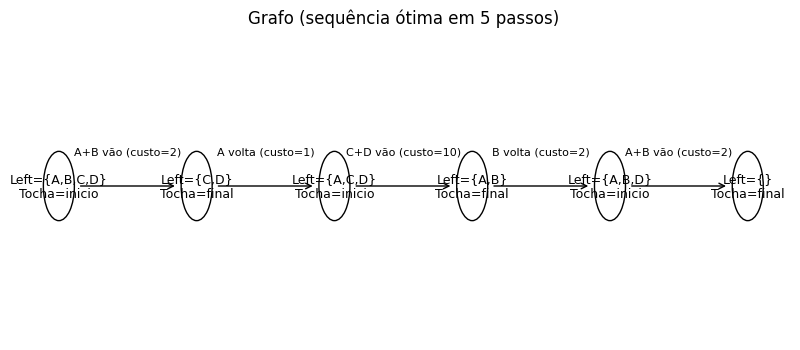
\includegraphics[width=0.8\linewidth]{optimal_path}
    \caption{Grafo ilustrando a sequência ótima em 5 passos, com movimentos de ida e volta intercalados e custo total de 17 minutos.}
    \label{fig:cen1}
\end{figure}

Na Figura \ref{fig:cen2} apresenta-se um exemplo de ramificação do grafo de estados, mostrando duas escolhas possíveis de ida (A+B ou A+C) e os estados resultantes após o retorno da tocha. Essa ilustração evidencia a multiplicidade de caminhos que podem ser explorados durante a busca.

\begin{figure}[H]
    \centering
    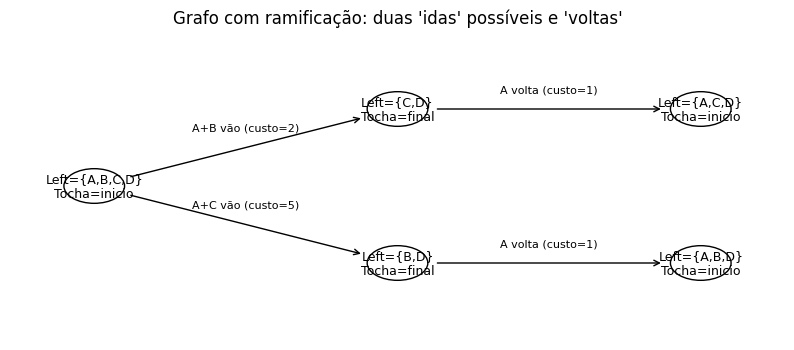
\includegraphics[width=0.8\linewidth]{ramification.png}
    \caption{Grafo com ramificação: duas possibilidades de ida e as respectivas voltas, mostrando a expansão do espaço de estados.}
    \label{fig:cen2}
\end{figure}

\subsection{Definição Formal do Grafo}
De forma resumida:
\begin{itemize}
\item \textbf{Vértices}: cada vértice corresponde a um estado $S = [p_1, p_2, p_3, p_4, t]$;
\item \textbf{Arestas}: cada aresta representa uma ação válida (ida ou volta de 1 ou 2 pessoas), com custo associado ao tempo da travessia;
\item \textbf{Justificativa}: essa modelagem é natural porque o espaço de estados é finito e discreto, permitindo a aplicação direta de algoritmos de busca como BFS e DFS;
\item \textbf{Exemplos ilustrativos}: os diagramas apresentados nas Figuras \ref{fig:cen1} e \ref{fig:cen2} ajudam a visualizar as transições de estados.
\end{itemize}


\section{Rotinas Desenvolvidas}
Explicar detalhadamente as rotinas implementadas.
\begin{itemize}
\item Estrutura geral do código;
\item Funções principais;
\item Decisões de implementação.
\end{itemize}

\section{Algoritmos de Busca Estudados}
Apresentar uma explicação básica dos algoritmos analisados.
\begin{itemize}
\item Busca em Largura (BFS);
\item Busca em Profundidade (DFS);
\item Outros algoritmos relevantes (caso aplicável).
\end{itemize}

\section{Comparação e Discussão dos Resultados}
Comparar os algoritmos aplicados para solucionar o puzzle.
\begin{itemize}
\item Critérios de comparação (tempo de execução, número de passos, consumo de memória, etc.);
\item Tabelas e gráficos com resultados;
\item Discussão dos pontos fortes e fracos de cada abordagem.
\end{itemize}

\section{Conclusão}
Apresentar as conclusões gerais do trabalho, destacando os principais aprendizados e possíveis melhorias futuras.

\section*{Referências}
\bibliographystyle{plain}
\bibliography{references}

\end{document}